% !TeX program = lualatex
% !TeX encoding = utf8
% !TeX spellcheck = uk_UA
% !TeX root = ../EMConspect.tex

%=========================================================
\chapter{Постійне електричне поле у вакуумі}\label{\currfilebase}
\graphicspath{{\currfilebase/Pictures}}
%=========================================================
\epigraph{\Alexander  ...взаємне тяжіння електричної рідини, іменованої позитивною, і електричної рідини, іменованої зазвичай негативною,
	полягає у зворотному відношенні квадратів відстаней...
}{Шарль Огюстен Кулон}


%% --------------------------------------------------------
\section{Сили (взаємодії) в природі}
%% --------------------------------------------------------

\emphx{Фізичні явища} базуються на взаємодії між тілами або частинками. Наприклад, рух Землі навколо Сонця викликаний гравітаційною взаємодією.
Притягання або
відштовхування електричних зарядів є проявом електричної взаємодії. Відштовхування чи притягання магнітних полюсів є проявом магнітної взаємодії. У XIX
столітті Джеймс Клерк Максвелл об’єднав електричну та магнітну взаємодії в електромагнітну. У мікросвіті існують ще дві взаємодії: слабка і сильна
ядерні. Сильна взаємодія утримує кварки в протонах і нейтронах, а також зв'язує їх у ядрах атомів. Слабка взаємодія відповідає за ядерні перетворення,
наприклад, бета-розпад (рис.~\ref{pic:interactions}).

\begin{figure}[h!]\centering
	
\includegraphics[width=\linewidth]{forces}
	\caption{Взаємодії в природі}
	\label{pic:interactions}
\end{figure}

Всі взаємодії передаються через поля. Наведемо цитату, яка влучно характеризує поняття поля:
\begin{tornpage}\small\itshape
	У фізиці з'явилося нове поняття, найважливіше досягнення з часу Ньютона: поле. Знадобилася велика наукова уява, щоб усвідомити собі, що не заряди і
	не  частинки, а поле в просторі між зарядами і частинками істотне для опису фізичних явищ.\\

	\hfill А. Ейнштейн, Л. Інфельд <<Еволюція фізики>>
\end{tornpage}

Основні типи фізичних полів:
\begin{enumerate}
	\item Гравітаційне поле забезпечує взаємодію між масами.
	\item Електромагнітне поле діє між зарядами та струмами.
	\item Глюонне поле відповідає за сильну взаємодію.
	\item Поле векторних бозонів опосередковують слабку взаємодію.
\end{enumerate}

Всі відомі взаємодії, від гравітаційної до ядерної, мають різну інтенсивність. Гравітація є найслабкішою з них, але інші взаємодії, такі як
електромагнітна, можуть бути надзвичайно сильними. Якщо ми розглянемо величину електричних сил, то побачимо справжній контраст. Наприклад, навіть
найменше порушення рівноваги між електронами та протонами може створити величезні сили. Річ у тім, що навіть невелика зміна кількості електронів може
призвести до таких ефектів, які здатні перевершити навіть гравітаційні сили на найглобальнішому рівні. І ось що про це говорить Річард Фейнман у своїх
лекціях з фізики:
\begin{tornpage}\small\itshape%\Alexander
	\hspace{\parindent}Якби у вашому тілі або в тілі вашого сусіда (який стоїть від вас на відстані витягнутої руки) електронів виявилося б всього на 1\%
	більше, ніж протонів, то сила вашого відштовхування була б неймовірно великою. Наскільки великою? Достатньою, щоб підняти хмарочос? Більше! Достатньою,
	щоб підняти гору Еверест? Більше! Сили відштовхування вистачило б, щоб підняти «вагу», що дорівнює вазі нашої Землі!\\

	\hfill{ Р. Фейнман в книзі <<Фейнманівські лекції з фізики>>}.
\end{tornpage}
%В основі всіх фізичних явищ лежить взаємодія між тілами або частинками, що беруть участь у цих явищах. Наприклад, Земля рухається навколо Сонця через
%гравітаційну взаємодію з ним. Іншим прикладом взаємодії є притягання або відштовхування електричних зарядів, яке є проявом електричної взаємодії.
%Відштовхування або притягання магнітних полюсів чи струмів --- це прояв магнітної взаємодії. У XIX столітті Джеймс Клерк Максвелл у своїй теорії
%об'єднав електричну та магнітну взаємодію. Це об'єднання отримало назву електромагнітної взаємодії.
%
%У мікросвіті, крім електромагнітної та гравітаційної взаємодій, діють ще два типи: слабка та сильна ядерні взаємодії. Сильна взаємодія утримує кварки
%всередині протонів і нейтронів, а також протони й нейтрони у ядрах атомів. Слабка взаємодія відповідає за ядерні перетворення, такі як бета-розпад.


%Всяка взаємодія передається через поле. Щоб зрозуміти це, слід звернути увагу на поняття <<далекодії>> та <<близькодії>>. У випадку далекодії взаємодія
%між тілами відбувається миттєво на будь-якій відстані, без явного посередника. Це уявлення панувало до XIX століття. Однак із розвитком фізики стало
%зрозуміло, що жодна взаємодія не може передаватися без проміжного агента. Таким агентом є поле. Земля взаємодіє із Сонцем через гравітаційне поле.
%Електричні заряди та струми взаємодіють через електромагнітне поле. Кварки в середині протона чи нейтрона взаємодіють через глюонне поле. А розпад
%протона, чи взаємодія електрона та нейтрино відбувається завдяки
%$W^{\pm}$- та $Z$-бозонним полям. Кожна частинка створює поле, і це поле вже діє на іншу частинку.
%
%
%Взаємодії у природі характеризуються кількома важливими властивостями: їхнім джерелом, ефектом, радіусом дії та інтенсивністю. Розглянемо ці аспекти
%детальніше, щоб зрозуміти основні відмінності між чотирма фундаментальними типами взаємодій.
%
%\emphx{Джерело взаємодії.} Кожна взаємодія виникає завдяки певним властивостям матерії. Наприклад, гравітаційна взаємодія обумовлена масою,
%електромагнітна --- електричним зарядом, слабка ядерна --- слабким зарядом, а сильна ядерна --- кольоровим зарядом кварків.
%
%\emphx{Ефект взаємодії.} Ця характеристика описує, як взаємодія впливає на тіла або частинки. Гравітація змушує всі тіла притягуватися одне до одного.
%Електромагнітна взаємодія може викликати як притягання, так і відштовхування залежно від знаків зарядів. Слабка ядерна взаємодія спричиняє ядерні
%перетворення, тоді як сильна взаємодія утримує кварки разом у складі протонів і нейтронів.
%
%\emphx{Радіус дії.} Ця властивість визначає, на якій відстані взаємодія залишається відчутною. Гравітація та електромагнітна взаємодія діють на
%необмежених відстанях, хоча їхній вплив слабшає із зростанням відстані. Слабка та сильна ядерні взаємодії мають дуже обмежений радіус дії, що становить
%$10^{-16}$ см і $10^{-13}$ см відповідно.
%
%\emphx{Інтенсивність.} Інтенсивність показує силу взаємодії. Гравітація є найслабшою з усіх типів взаємодій, тоді як сильна ядерна взаємодія є
%найпотужнішою. Електромагнітна взаємодія займає проміжне місце між цими крайнощами, а слабка ядерна взаємодія за своєю інтенсивністю перевищує
%гравітацію, але значно поступається електромагнітній і сильній.
%
%Для зручності всі ці характеристики зібрано в таблицю~\ref{tab:forces}.



Звичайні сили, які виникають під час зіткнення предметів (рука і камінь, підошва і земля), пояснюються електромагнітною взаємодією. Атоми дотичних тіл
зближуються на відстань порядку атомних розмірів, і їхні електрони та ядра створюють електромагнітне поле, яке забезпечує взаємодію. Ця ж взаємодія
утримує атоми разом, забезпечуючи існування твердих і рідких тіл.

%\emphx{Електромагнітна взаємодія} є одним із фундаментальних типів
%взаємодій і передається за допомогою агента ---
%\emphx{електромагнітного поля}.
%
%\emphx{Електромагнітним полем} називається область простору, де діють
%електричні та магнітні сили.

%Поле \emphx{створюється} електричними \textit{зарядами} і \emphx{діє}
%на \textit{заряди}.


\section{Електричний заряд}

\emphx{Електричний заряд} --- це міра взаємодії \emphx{зарядженого
	тіла з полем}. Фактично, заряд визначає інтенсивність взаємодії
заряджених тіл.

\begin{Attention}
	Заряд --- фундаментальна властивість деяких видів елементарних
	частинок.
\end{Attention}

%\begin{wrapfigure}[12]{r}{0.3\linewidth}\centering
%	
\includegraphics[width=\linewidth]{Millikan-chamber}
%	\caption{Установка Міллікена}
%\end{wrapfigure}

Експеримент із вимірювання елементарного електричного заряду,
здійснений 1909 року Робертом Ендрюсом Міллікеном та Гарві
Флетчером. В результаті було встановлено дискретність електричного
заряду та визначив величину заряду електрона з точністю до 1\%.
%\href{https://www.youtube.com/watch?v=5LC4-ct_1-M}{Відео: Досліди Міллікена та Йоффе}




\begin{enumerate}
	\item Дискретність заряду.

	      Дослідним шляхом було встановлено, що в природі існують \emphx{заряди двох типів}, які умовно ділять на \emphx{позитивні} та
	      \emphx{негативні}. Позитивний заряд несуть, наприклад, протони, а негативний --- електрони. У природі заряд змінюється (переноситься) дискретно, причому
	      будь-який ненульовий заряд кратний деякому елементарному заряду, що чисельно дорівнює заряду електрона:
	      \begin{equation*}
		      e = 4.803 \cdot 10^{-10}\ \text{Фр} = 1.602 \cdot 10^{-19}\ \text{Кл}.
	      \end{equation*}

%    \item Адитивність заряду. Заряд є адитивною величиною. Це означає

	\item Збереження заряду.

	      Заряд --- це величина, що \emphx{зберігається}. Позитивні й негативні заряди можуть народжуватися в рівних кількостях або взаємно
	      знищувати один одного. При цьому сумарний електричний заряд речовини не змінюється.
	\item Релятивістська інваріантність заряду.

	      Величина електричного заряду однакова відносно різних систем відліку. Іншими словами, величина заряду не залежить від швидкості.
\end{enumerate}



\section{Як заряджають тіла?}

%	\tikz[remember picture,overlay] \node[opacity=0.7,inner sep=0pt,
%		anchor=south east] at (current page.south
%	east){
\includegraphics[width=3cm]{Tribocat}};
%
%	\tikz[remember picture,overlay] \node[opacity=0.7,inner sep=0pt,
%		anchor=north west] at ([yshift=-1.5cm]current page.north
%	west){
\includegraphics[width=5cm]{charging-by-friction}};
%
%	\tikz[remember picture,overlay] \node[opacity=0.7,inner sep=0pt,
%		anchor=north east] at ([yshift=-1.7cm]current page.north
%	east){
\includegraphics[width=3cm]{Amber}};

\emphx{Трибоелектричний ефект} --- поява електричних зарядів у
матеріалі через тертя (рис.~\ref{pic:triboeffect}).

Деякі матеріали стають електрично зарядженими після того, як вони
входять у фрикційний контакт з іншим матеріалом.

%---------------------------------------------------------
\begin{SCfigure}[][h!]
	%\begin{minipage}{0.35\linewidth}
	%    \centering
	%    
\includegraphics[height=3cm]{Amber}
	%    \caption{Шматок бурштину}
	%\end{minipage}
	%\quad
	%\begin{minipage}{0.65\linewidth}
	\centering
	
\includegraphics[height=3cm]{charging-by-friction}
	\caption{Електризація тертям\label{pic:triboeffect}}
	%\end{minipage}
\end{SCfigure}
%---------------------------------------------------------

Слово <<\emphx{електрика}>> походить від грецького
<<$\eta\lambda\varepsilon\kappa\tau\rho o \nu$>>
(\emphx{електрон}), що означає <<\emphx{бурштин}>>. Люди помітили,
що бурштин, натертий об хутро, притягує дрібні предмети, і це
явище згодом стало основою для дослідження електричних явищ.



Матеріали, що виявляють трибоелектричний ефект, прийнято
розташовувати в \emphx{трибоелектричний ряд}, один кінець якого є
позитивним, а інший --- негативним. Під час тертя пари матеріалів
з ряду, матеріал, розташований ближче до позитивного кінця ряду,
зарядиться позитивно, а інший --- негативно (рис.~\ref{tikz:triboseries}).


\begin{figure}[h!]
	\centering
	\begin{tikzpicture}
		% Градієнт фону
		\shade[left color=blue!30, right color=red!30] (-5.5, -.5) rectangle (5.5, -3.5);

		\node[single  arrow, single  arrow head extend=.5cm, left color=blue!50, right color=red!50, text=white, font={\bf \large}, inner sep=0.3cm]
		(doublearrow)
		{--\hspace*{10.5cm}+};

		% Трибоелектричний ряд
		\node[align=center, rotate=90] at (5,  -2) {Хутро};
		\node[align=center, rotate=90] at (4,  -2) {Фланель};
		\node[align=center, rotate=90, align=center, text width=2.5cm] at (3,  -2) {Слонова\\ кістка};
		\node[align=center, rotate=90] at (2,  -2) {Пір'я};
		\node[align=center, rotate=90] at (1,  -2) {Флінтглас};
		\node[align=center, rotate=90] at (0,  -2) {Шовк};
		\node[align=center, rotate=90] at (-1, -2) {Алюміній};
		\node[align=center, rotate=90] at (-2, -2) {Поліестер};
		\node[align=center, rotate=90] at (-3, -2) {Папір};
		\node[align=center, rotate=90] at (-4, -2) {Бурштин};
		\node[align=center, rotate=90] at (-5, -2) {Ебоніт};
	\end{tikzpicture}
	\caption{Трибоелектричний ряд\label{tikz:triboseries}}
\end{figure}


%% --------------------------------------------------------
\section{Взаємодія нерухомих зарядів}
%% --------------------------------------------------------


%% --------------------------------------------------------
\subsection*{Закон Кулона}
%% --------------------------------------------------------
Експериментально встановлено, що заряди одного знака (однойменні
заряди) \emphx{відштовхуються}, а заряди різного знака (різнойменні
заряди) --- \emphx{притягуються}.


\emphx{Точковим} називається такий заряд, розмірами та формою якого в
умовах, що розглядаються, можна знехтувати.


Закон, установлений Ш. Кулоном у 1785 р., стверджує, \emphx{що сила,
	що діє на точковий заряд} $q_1$ з боку точкового заряду $q_2$:
\begin{equation}\label{eq:ColumbLaw}
	\tcbhighmath{
		\vect{F}_{12} = \frac{q_1 q_2}{r^2}\frac{\vect{r}_{12}}{r}.
	}
\end{equation}


\begin{SCfigure}[0.5][h!]
	\centering
	\localinput{Columb.tikz}
	\caption{Ілюстрація до закону Кулона}
\end{SCfigure}


%% --------------------------------------------------------
\subsection*{Експериментальні перевірки закону Кулона}
%% --------------------------------------------------------


Якщо припустити, що закон взаємодії точкових зарядів відрізняється від закону оберненого квадрату, наприклад:
\begin{equation*}
	F = \frac{q_1 q_2}{r^{2 + \epsilon}},
\end{equation*}
де $|\epsilon| \ll 1$, то при збереженні принципу суперпозиції це призводить до якісних змін у поведінці зарядів у
провідниках. У випадку кулонівської взаємодії у стаціонарних умовах заряди зосереджуються на поверхні провідника, а всередині зарядів немає.
Однак, якщо виконується формула з $\epsilon$, то можна показати, що у провіднику виникає ненульова густина заряду у стаціонарних умовах.

\begin{SCfigure}[0.75][h!]
	\centering
	
\includegraphics[width=0.5\linewidth]{cavindesh_exp}
	\caption{Установка Г.~Кавендіша для перевірки закону обернених квадратів.}
	\label{pic:Cavendih_exp}
\end{SCfigure}

Цю обставину було використано Г.~Кавендішем для отримання обмеження на $\epsilon$ (рис.~\ref{pic:Cavendih_exp}). На попередньо заряджену провідну кулю
накладали дві провідні напівсфери, які щільно прилягали одна до одної, утворюючи майже суцільну поверхню. У цій системі, у разі кулонівської взаємодії
($\epsilon = 0$), весь заряд переходить на зовнішні напівсфери. Якщо ж $\epsilon \neq 0$, всередині кулі залишається заряд (тим менший, чим менше
$\epsilon$), який можна
виміряти за допомогою чутливого електрометра після зняття напівсфер. Цей експеримент неодноразово повторювався із поступовим підвищенням точності. У
1983 році було отримано обмеження:
\begin{equation*}
	|\epsilon| < 10^{-16} \text{–} 10^{-17}.
\end{equation*}



%% --------------------------------------------------------
\section{Електричне поле}
%% --------------------------------------------------------

У законі Кулона заряди взаємодіють на відстані один від одного, однак виникає питання: як ці заряди відчувають один одного?

Історично існувало два протилежні підходи до відповіді на поставлені запитання. При одному з них передбачалося, що тілам притаманна властивість діяти на
інші тіла на відстані, без участі проміжних тіл або середовища і сили можуть передаватися від
одного тіла до іншого через вакуум миттєво (теорії далекодії).

Відповідно до теорії близькодії, взаємодія між тілами передається через певне середовище, яке їх оточує, і поширюється послідовно від однієї частини
цього середовища до іншої. Досліди показують, що цей підхід є фізично обґрунтованим, а сама взаємодія передається з кінцевою швидкістю, що
узгоджується з сучасними уявленнями про природу фізичних процесів.


  Для пояснення взаємодії заряджених тіл вводять поняття
\emphx{електричного поля}. Воно виникає навколо заряджених тіл і є особливим видом матерії. Його головна властивість --- здатність діяти на інші
заряди, що потрапляють у цю область. Тобто, електричне поле є матеріальним посередником у передачі сил між зарядами, забезпечуючи локальний характер
взаємодії: взаємодія поля і заряду відбувається в одній і тій же точці простору.



%% --------------------------------------------------------
\subsection*{Напруженість поля та принцип суперпозиції}
%% --------------------------------------------------------



Для дослідження поля, створюваного будь-якими зарядами (зарядженими тілами), можна використовувати \emphx{пробні заряди}.

\emphx{Пробним} називається такий невеликий за величиною точковий заряд, який не спричиняє помітного перерозподілу зарядів, що створюють досліджуване
поле.


Дослідним шляхом установлено, що якщо помістити в електричне поле пробний заряд $q$ то відношення сили $\vect{F}$, що діє на цей заряд, до величини
заряду не залежить від величини заряду. Отже, відношення $\vect{F}/q$ характеризує поле, але не заряд. Цю характеристику називають \emphx{напруженістю
електричного поля}:
\begin{equation}\label{eq:E}
	\tcbhighmath{\Efield = \frac{\vect{F}}{q}.}
\end{equation}
Напруженість --- є силовою характеристикою електричного поля.

Поняття напруженості поля ґрунтується на теорії близькодії, тобто, на пробний заряд діє сила не з боку інших заряджених тіл, а збоку поля в тій же
точці, де знаходиться пробний заряд (рис.~\ref{tikz:F=qE}). Ця сила дорівнює:
\begin{equation}
    \vect{F} = q\Efield(\vect{r}),
\end{equation}
де $\vect{r}$ --- радіус-вектор, що задає положення заряду.


\begin{SCfigure}[1.5][h!]
	\centering
    \begin{tikzpicture}[>=latex, scale=1.5]

        \coordinate (O) at (0.5,-0.5);

       	\draw[->] (O) -- ++(1, 0) node[below] {$y$};
       	\draw[->] (O) -- ++(0, 1) node[above] {$z$};
       	\draw[->] (O) -- ++(-135:0.75) node[below] {$x$};

        \draw[midarrow, red] (1.24,0) to[bend left] ++(75:3);
        \draw[midarrow, red, tangent=0.2] (1.6,0) to[bend left=20pt] ++(70:3);
        \draw[use tangent=1, ->, ultra thick, cyan] (0, 0) node[circle, ball color=red, inner sep=1pt, text=white, font=\scriptsize] (q) {} --
        ++(2,0)
        node[right, pos=0.5, text=black]
        {$q\Efield(\vect{r})$};
        \draw[->] (O) -- node[left] {$\vect{r}$} (q);
        \draw[midarrow, red] (1.86,0) to[bend left=20pt] ++(55:3);

    \end{tikzpicture}
	\caption{Сила, що діє з боку поля на заряд $q$ відбувається в одній і тій же точці простору (носить локальний характер) і дорівнює $\vect{F} =
	q\Efield$.}
    \label{tikz:F=qE}
\end{SCfigure}

Нехай положення точкового заряду  $Q$, що створює поле, задається радіус-вектором $\vect{r}'$. Із закону Кулона можна легко знайти напруженість, як
функцію точки спостереження, яка задається радіус-вектором $\vect{r}$ (рис.~\ref{tikz:E}):
\begin{equation}
	\tcbhighmath{
		\Efield(\vect{r}) = \frac{Q}{|\vect{r} - \vect{r}'|^2}\ \frac{\vect{r} - \vect{r}'}{|\vect{r} - \vect{r}'|}.
	}
\end{equation}

\begin{SCfigure}[0.7][h!]
	\centering
\begin{tikzpicture}[>=latex,
                chp/.style = {circle, inner sep=1pt, ball color=red,  font=\tiny\mathstrut, text=white, inner sep=0pt},
                chn/.style = {circle, inner sep=1pt, ball color=blue, font=\tiny\mathstrut, text=white, inner sep=0pt},
]
    \coordinate (O) at (-1, -0.5, 0);
	\draw[->] (O) -- ++(0, 2, 0) node[above] {$z$};
	\draw[->] (O) -- ++(0, 0, 4) node[left]  {$x$};
	\draw[->] (O) -- ++(2, 0, 0) node[below] {$y$};

    \pgfmathsetseed{42}

    \node[chp] (q) at (0.5,1.8,1)  {$+$};
    \node[above=6pt] at (q) {$Q$};

	\node[circle, inner sep=0.5, fill] (P) at (xyz polar cs:angle=45, x radius=7, y radius=3) {};

    \draw[->, red] (O) --  (q) node[anchor=east, text=black, pos=0.6, inner sep=1pt] {$\vect{r}'$};
    \draw[->, blue] (q) -- node[above, sloped] {$\vect{r} - \vect{r}'$} (P);
    \draw[->] (O) -- (P) node[below, sloped, pos=0.8] {$\vect{r}$} ;
   	\node[below] at (P) {$P$};
    \draw[->, red, thick] (P) -- ($(q)!1.2!(P)$) node[above] {$\Efield(\vect{r})$};
\end{tikzpicture}
	\caption{Напруженість поля точкового заряду $Q$}
    \label{tikz:E}
\end{SCfigure}


Напруженість поля заряджених тіл складної геометричної форми можна знайти за принципом суперпозиції.

Розглянемо електричне поле двох точкових зарядів $q_1$ і $q_2$. Нехай $\Efield_1$ --- напруженість поля в точці а, створювана зарядом $q_1$ (коли
заряду $q_2$ немає зовсім), а $\Efield_2$ --- напруженість поля заряду $q_2$ (коли немає заряду $q_1$). Дослід показує, що напруженість $\Efield$
результуючого поля (за наявності обох зарядів) може бути знайдена за правилом додавання векторів (рис.~\ref{tikz:Superposition}).

\begin{SCfigure}[][h!]
	\centering
	\localinput{Superposition.tikz}
	\caption{Ілюстрація принципу суперпозиції для випадку двох різнойменних зарядів}
    \label{tikz:Superposition}
\end{SCfigure}

Правило векторного додавання електричних полів справедливе не тільки для двох, а й для будь-якої системи зарядів. Якщо $\Efield_1$, $\Efield_2$,
\ldots, $\Efield_n$ --- напруженості полів, створюваних окремими зарядами в якій-небудь точці, то напруженість $\Efield$ результуючого поля в тій самій
точці дорівнює:
\begin{equation}
	\Efield = \sum_{i=1}^{n} \Efield_i,
\end{equation}
це співвідношення виражає \emphx{принцип суперпозиції електричних полів} і являє собою важливу властивість електричного поля.

Якщо заряди розподілені неперервно, то принцип суперпозиції буде мати вигляд:
\begin{equation}
	\Efield = \int d\Efield,
\end{equation}
де де $d\Efield$ -- напруженість електричного поля, створювана елементарним зарядом $dq$, а інтегрування ведеться за всією областю, в якій розподілені
заряди. Для різних типів розподілів використовуються відповідні диференціальні елементи заряду:

\begin{itemize}
\item Для лінійного розподілу: $dq = \lambda , dl$, де $\lambda$ --- лінійна густина заряду, $dl$ — елемент довжини.
\item Для поверхневого розподілу: $dq = \sigma , dS$, де $\sigma$ --- поверхнева густина заряду, $dS$ — елемент площі.
\item Для об'ємного розподілу: $dq = \rho , dV$, де $\rho$ --- об'ємна густина заряду, $dV$ — елемент об'єму.
\end{itemize}

В разі об'ємного розподілу напруженість поля визначається як:
\begin{equation}
    \Efield(\vect{r}) = \iiint\limits_V \frac{\rho(\vect{r}')dV'}{|\vect{r} - \vect{r}'|^2}\ \frac{\vect{r} - \vect{r}'}{|\vect{r} - \vect{r}'|}.
\end{equation}


\begin{SCfigure}[0.65][h!]
% Размер куба
\def\cx{.33} % относительный размер куба

% Создание стиля узла для куба
\tikzset{
  cube/.style={
    append after command={
      \pgfextra{
        % Сторона сверху
        \fill[#1!20, draw=#1]
          (\tikzlastnode.south west) --
          ($(\tikzlastnode.south west) + (\cx,0,0)$) --
          ($(\tikzlastnode.south west) + (\cx,\cx,0)$) --
          ($(\tikzlastnode.south west) + (0,\cx,0)$) --
          cycle;
        % Передняя сторона
        \fill[#1!10, draw=#1]
          ($(\tikzlastnode.south west) + (0,\cx,0)$) --
          ($(\tikzlastnode.south west) + (0,\cx,-\cx)$) --
          ($(\tikzlastnode.south west) + (\cx,\cx,-\cx)$) --
          ($(\tikzlastnode.south west) + (\cx,\cx,0)$) --
          cycle;
        % Правая сторона
        \fill[#1!30, draw=#1]
          ($(\tikzlastnode.south west) + (\cx,0,0)$) --
          ($(\tikzlastnode.south west) + (\cx,\cx,0)$) --
          ($(\tikzlastnode.south west) + (\cx,\cx,-\cx)$) --
          ($(\tikzlastnode.south west) + (\cx,0,-\cx)$) --
          cycle;
      }
    }
  }
}
\begin{tikzpicture}[>=latex]
    \coordinate (O) at (-1, -0.5, 0);
	\draw[->] (O) -- ++(0, 2, 0) node[above] {$z$};
	\draw[->] (O) -- ++(0, 0, 4) node[left]  {$x$};
	\draw[->] (O) -- ++(2, 0, 0) node[below] {$y$};

    \pgfmathsetseed{42}
    \fill[gray, opacity=0.5] (0.5, 0.5, 0) plot[domain=0:360, smooth cycle] ({\x}:{0.2*rnd + 1.7});

    \node[cube=red] (q) at (0.5,1.8,1)  {};
    \node[above=6pt] at (q) {$\rho(\vect{r}') dV'$};

	\node[circle, inner sep=0.5, fill] (P) at (xyz polar cs:angle=45, x radius=7, y radius=3) {};

    \draw[->, red] (O) --  (q) node[anchor=east, text=black, pos=0.6, inner sep=1pt] {$\vect{r}'$};
    \draw[->, blue] (q) -- node[above, sloped] {$\vect{r} - \vect{r}'$} (P);
    \draw[->] (O) -- (P) node[below, sloped, pos=0.8] {$\vect{r}$} ;
   	\node[below] at (P) {$P$};
    \draw[->, red, thick] (P) -- ($(q)!1.2!(P)$) node[above] {$d\Efield(\vect{r})$};
\end{tikzpicture}
\caption{До розрахунку електричного поля за принципом суперпозиції у разі об'ємного розподілу заряду.}
\label{tikz:superposition_for_E}
\end{SCfigure}

\begin{problem}%
Тонкий довгий стрижень рівномірно заряджений з лінійною густиною $\lambda = 10$~мкКл/м. На продовженні осі стрижня на відстані $l = 20$~см від
його кінця знаходиться точковий заряд $q = 10$~нКл. Визначити силу взаємодії зарядженого стрижня і точкового заряду.
\end{problem}

\begin{problem}%
Нехай є тонкий диск радіуса $R$, поверхнею якого рівномірно розподілено
заряд $Q$. Знайти електричне поле на осі диска на відстані $z$ від його
площини.
\begin{center}
	\localinput{DiskField.tikz}
\end{center}
\end{problem}


%% --------------------------------------------------------
\subsection*{Силові лінії}
%% --------------------------------------------------------

%Для того щоб описати електричне поле, потрібно задати вектор напруженості в кожній точці поля. Це можна зробити аналітично, виражаючи залежність
%напруженості поля від координат у вигляді формул.
%
%
%Однак цю залежність можна представити й графічно. Для цього користуються силовими лініями. \emphx{Силовою лінією}, або лінією вектора напруженості
%поля,
%називають лінію, проведену в електричному полі, для якої напрямок дотичної в будь-якій точці збігається з напрямком вектора напруженості поля
%(рис.~\ref{tikz:force_line}). Оскільки дотична, як і будь-яка пряма, визначає два взаємно протилежні напрямки, то силовій лінії приписують певний
%напрямок, відзначаючи його на рисунку стрілкою. Щоб за допомогою силових ліній зобразити не тільки напрямок, а й величину напруженості поля, домовилися
%на графіках поля проводити силові лінії з певною густотою, а саме так, щоб кількість силових ліній, які проходять через одиницю поверхні,
%перпендикулярної до силових ліній, дорівнювала (або була пропорційною) величині напруженості поля в даному місці. Зображуючи силові лінії поля, ми
%отримуємо своєрідні графіки або карти поля, які відразу наочно показують, чому дорівнює напруженість у різних частинах поля і як вона змінюється в
%просторі.

Електричне поле можна описати за допомогою вектора напруженості, який задають аналітично (формулами) або графічно через силові лінії.

\emphx{Силова лінія} --- це лінія, дотична до якої в кожній точці збігається з напрямком вектора напруженості (рис.~\ref{tikz:force_line}). Їй надають
напрямок, позначаючи стрілкою.

\begin{SCfigure}[2][h!]
	\centering
	\localinput{fieldlines.tikz}
	\caption{Вектори $\Efield$ є дотичними до силової лінії}
    \label{tikz:force_line}
\end{SCfigure}

Густота силових ліній пропорційна величині напруженості: чим більша напруженість, тим більше ліній перетинають одиницю площі, що перпендикулярна до них.

Зображуючи силові лінії поля, ми отримуємо своєрідні графіки або карти поля, які відразу наочно показують, чому дорівнює напруженість у різних частинах
поля і як вона змінюється в просторі.



Вигляд картини силових ліній можна отримати в \href{https://www.youtube.com/watch?v=KDEjgCEy2LU}{експерименті} занурюючи електроди ванну, заповнену
суспензією манної крупи в касторовій олії.

Аналітично також можна розрахувати вигляд силових ліній. Оскільки елемент лінії $d\vect{\ell}$ в кожній точці паралельний до вектора напруженості, то
вводячи деякий неособливий параметр $p$, можна записати диференціальне рівняння:
\begin{equation}
    d\vect{\ell} = p\Efield,
\end{equation}
або в проекціях:
\begin{equation*}
    \frac{dx}{E_x} = \frac{dy}{E_y} = \frac{dz}{E_z}.
\end{equation*}


На рис.~\ref{pic:force_line} як приклад наведено картину силових ліній пари точкових зарядів.


\begin{figure}[h!]
	\centering
	\includegraphics[width=0.75\linewidth]{fieldlines}
	\caption{Вигляд силових ліній системи двох зарядів}
    \label{pic:force_line}
\end{figure}




%%% --------------------------------------------------------
\section{Теорема Гаусса для електричного поля у вакуумі}
%%% --------------------------------------------------------


%% --------------------------------------------------------
\subsection*{Нові поняття}
%% --------------------------------------------------------

Чи достатньо закону Кулона і принципу суперпозиції для визначення
напруженості електричного поля довільної системи зарядів?

Для простих випадків вони є ефективними \emphx{інструментами для обчислення електричного поля} системи зарядів, або поля заряджених тіл складної
геометричної форми. Проте, є випадки, коли геометрією розподілу зарядів така, що аналітичні розрахунки виконати не можна. Тому в теорії поля були
\emphx{введені допоміжні концепції та методи}, які \emphx{спрощують обчислення і аналіз} полів у складних системах, дозволяючи ефективніше проаодити
аналіз та  вирішувати  задачі аналітично.


\begin{Attention}\small
Наприклад, спробуйте обчислити за допомогою закону Кулона і принципу
суперпозиції напруженість поля всередині рівномірно зарядженої кулі. Вийде
так, що інтеграли буде практично неможливо вирішити аналітичним методом.
Чисельно (на комп'ютері), це зробити можна, але чисельні результати не
можна якісно проаналізувати.
\end{Attention}

 Далі вводяться нові концепції та методи, які дадуть змогу це робити.

%% --------------------------------------------------------
\subsection*{Потік вектора швидкості}
%% --------------------------------------------------------

Поняття потоку прийшло з гідродинаміки, де течію рідини можна розглядати як поле вектора швидкості $\vect{v}$.
Порахуємо об'єм рідини $dV$, що протікає за час $dt$ через поверхню~$S$ (рис.~\ref{tikz:Flux}).

%---------------------------------------------------------
\begin{figure}[h!]\centering
	\localinput{Phi.tikz}
	\caption{До виведення поняття потоку вектора}
    \label{tikz:Flux}
\end{figure}
%---------------------------------------------------------

З геометрії рисунка видно, що:
\begin{equation*}
	\frac{dV}{dt} = \frac{S d\ell \cos\theta}{dt} = \frac{d\ell}{dt} S\cos\theta = v_n S = \vect{v} \cdot \vect{n}\ S = \vect{v} \cdot \vect{S},
	\quad
	\vect{S}
	= \vect{n}S
\end{equation*}

Об'єм рідини, що протікає за одиницю часу $dV/dt = \Phi$ через поверхню~$S$ виражається через скалярний добуток вектора швидкості $\vect{v}$ і вектора
площі $\vect{S}$ і називається \emphx{потоком вектора швидкості}!

\begin{minipage}{0.35\linewidth}
	\localinput{SurfaceV.tikz}
\end{minipage}
\begin{minipage}{0.6\linewidth}
	Для довільної (не обов'язково плоскої) поверхні потік через елементарну
	площадку $d\Phi = v_n dS = \vect{v}\cdot d\vect{S}$. А через всю поверхню~$S$:
	\begin{equation*}
		\Phi = \iint\limits_S \vect{v}\cdot d\vect{S}
	\end{equation*}
\end{minipage}



%% --------------------------------------------------------
\subsection*{Потік вектора $\Efield$}
%% --------------------------------------------------------

\begin{minipage}{0.4\linewidth}
	\localinput{SurfaceE.tikz}
\end{minipage}
\begin{minipage}{0.6\linewidth}\centering

	\begin{tikzpicture}[scale=1, >=latex, midarrow/.style={%
					postaction={ decorate,
							decoration={ markings, mark=at position .7 with
										{\arrow{stealth}}}}}]

		\foreach \y in {-4,...,4}{
				\draw[red, midarrow, line width=0.5pt] plot[domain=0.5:6] (\x,
				0.2*\y+0.01*\y*\x^2);
			}

		\node[] at (4,-1.6)
		{
\includegraphics[width=0.4\linewidth]{butterflynet}};
	\end{tikzpicture}

\end{minipage}


Потік вектора $\Efield$ через елементарну площадку $dS$:
\begin{equation*}
	d\Phi = E_n dS = \Efield\cdot d\vect{S}.
\end{equation*}



Інтеграл
\begin{equation}
	\Phi = 	\iint\limits_S \Efield\cdot d\vect{S} = \iint\limits_S E_n\ dS
\end{equation}
називають \emphx{потоком вектора напруженості електричного поля} $\Efield$ через поверхню
$S$, хоча з цим поняттям і не пов'язана жодна реальна течія.

Потік --- величина скалярна: вона залежить не тільки від конфігурації поля $\Efield$, а й від вибору напрямку нормалі. У випадку замкнутих поверхонь
прийнято нормаль $\vect{n}$ брати назовні області, що охоплюється цими поверхнями, тобто \emphx{вибирати зовнішню нормаль}, що надалі буде завжди і
матися на увазі.


%% --------------------------------------------------------
\subsection*{Теорема Гаусса}
%% --------------------------------------------------------

Потік вектора $\Efield$ крізь довільну замкнуту поверхню $S$ має таку властивістю, що він залежить тільки від сумарного
заряду, що охоплюється цією поверхнею:

\begin{equation}\label{eq:GaussThm}\tag{\theequation a}
	\tcbhighmath{
		\oiint\limits_{\tikzmarknode{S}{S}} \Efield\cdot
		d\vect{S} =
		4\pi \sum\limits_i q_i,
	}
\end{equation}
де кружок біля інтеграла нагадує нам, що інтегрування проводиться по замкнутій поверхні $S$.  Це твердження носить назву \emphx{теореми Гаусса}.

\begin{SCfigure}[1][h!]
    \centering
	\localinput{GaussThm.tikz}
    \caption{Ілюстрація до доведення теореми Гаусса. \\ {\small На рисунку показано заряд в всередині замкненої поверхні $S$. На поверхні показано
    довільний елемент $d\vect{S}$ і кут між ним та напрямом вектора $\Efield$.}}
    \label{tikz:Gauss_thm}
\end{SCfigure}

Доведемо теорему. Спочатку розглянемо поле одного точкового заряду $q$. Оточимо цей заряд довільною
замкнутою поверхнею $S$ (рис.~\ref{tikz:Gauss_thm}) і знайдемо потік вектора $\Efield$
крізь елемент $d\vect{S}$:
\begin{equation*}
    d\Phi = \Efield\cdot d\vect{S} = E dS\cos\alpha = \frac{q}{r^2} dS \cos\alpha = q d \Omega.
\end{equation*}
де $d \Omega $ --- тілесний кут, що спирається на елемент поверхні $dS$, з вершиною в точці розташування заряду $q$. Інтегрування
цього виразу по всій поверхні $S$ еквівалентно інтегруванню по всьому тілесному куту $\Phi  = \int d\Phi = \int q d\Omega = 4\pi q$, як і вимагає
\eqref{eq:GaussThm}.

Коли заряди розподілені неперервно з об'ємною густиною $\rho(x,y,z)$, що залежить від координат, можна
вважати, що кожен елементарний об'єм $dV$ містить <<точковий>> заряд $\rho dV$. Тоді в правій частині \eqref{eq:GaussThm}:
\begin{equation*}
    q_V = \iiint\limits_V \rho dV,
\end{equation*}
де інтегрування проводиться тільки за об'ємом, який оточується замкнутою поверхнею $S$, тоді
\begin{equation}\tag{\theequation б}
	\tcbhighmath{
		\oiint\limits_{\tikzmarknode{S}{S}} \Efield\cdot
		d\vect{S} =
		4\pi \iiint\limits_{\tikzmarknode{V}{V}} \rho dV.
	}
\tikz[remember picture, overlay]{\draw[-latex,red] (V.south west)
	to[bend left] (S.south east);}
\end{equation}

Стрілка в цій формулі нагадує, що об'єм $V$ охоплюється замкненою поверхнею~$S$.

\begin{Attention}
Для розрахунку електричних полів системи зарядів теореми Гаусса
	недостатньо, бо вона є скалярним співвідношенням, чого
замало для визначення трьох невідомих --- складових $E_x$, $E_y$, $E_z$
вектора $\Efield$. \emphx{Необхідна відома симетрія задачі}, щоб остання
звелася до розв'язання одного скалярного рівняння.
\end{Attention}


\begin{problem}%
Визначити напруженість поля $\Efield$ усередині та поза безмежним плоским шаром товщини $d$, у якому рівномірно розподілений позитивний заряд з об'ємною
густиною $\rho$.
\end{problem}


%% --------------------------------------------------------
\subsection*{Теорема Ерншоу}
%% --------------------------------------------------------

Нехай у вакуумі є система нерухомих точкових зарядів, що перебувають у рівновазі.
Розглянемо один із цих зарядів --- заряд $q$. Чи може стан його рівноваги бути стійким?


\begin{wrapstuff}[type=figure, width=0.3\linewidth, o, top=2]
    \centering
    \localinput{Ernshow.tikz}
    \caption{До теореми Ерншоу}%
    \label{tikz:irnshow}
\end{wrapstuff}
Оточимо заряд $q$ невеликою замкнутою поверхнею $S$ (рис.~\ref{tikz:irnshow}). Нехай, для визначеності, $q > 0$. Для того, щоб рівновага заряду $q$ була
стійкою, необхідно, щоб у всіх точках поверхні $S$ поле $\Efield$, утворене всіма іншими зарядами системи, було спрямоване до заряду $q$: тільки в цьому
разі за будь-якого малого зсуву заряду $q$ з положення рівноваги на нього діятиме сила, яка повертатиме його назад, і положення рівноваги справді буде
стійким. Але така конфігурація поля $\Efield$ навколо заряду $q$ суперечить теоремі Гауса: потік вектора $\Efield$ крізь поверхню $S$ є від'ємним,
згідно ж з теоремою Гауса він має дорівнювати нулю, оскільки цей потік створюється зарядами, розташованими поза поверхнею $S$. А рівність потоку вектора
$\Efield$ нулю означає, що в якихось точках поверхні $S$ вектор $\Efield$ спрямований усередину, а в якихось обов'язково назовні. Звідси ипливає, що
\emphx{стійка рівновага заряду в будь-якому електростатичному полі неможлива}. Це твердження носить назву \emphx{теореми Ерншоу}. Вона, як видно з
вищесказаного, є наслідком теореми Гаусса. Теорему можна ще сформулювати по іншому: \emphx{будь-яка рівноважна конфігурація точкових зарядів нестійка,
якщо на них окрім кулонівських сил не діють  інші сили}.

Важливим висновком із теореми Ерншоу є те, що два різнойменні заряди, наприклад, електрон і ядро атома, не можуть залишатися в стані спокою --- такої
стійкої конфігурації не існує. Електрона має якимось чином рухатись в атомі.


%% --------------------------------------------------------
\subsection*{Зв'язок скалярних та векторних полів у сусідніх точках \\ (математичні відомості)}
%% --------------------------------------------------------

Часто виникає необхідність визначити, як змінюється значення поля в околі певної точки. Для цього можна використати наближені вирази, які дозволяють
оцінити зміну значення поля для малих зсувів. У випадку скалярної функції однієї змінної, можна застосувати перший член ряду Тейлора, що дає вираз:
\begin{equation*}
	f(x + \epsilon) = f(x) + \frac{df}{dx}\epsilon, \quad \epsilon \to 0.
\end{equation*}

\begin{SCfigure}[][h!]%{O}{0.3\linewidth}
	\centering

	\localinput{mathinfinitesimal.tikz}

	\caption{Ілюстрація до формул. Функція-поле $f(\vect{r})$ і різних точках простору.}
\end{SCfigure}

Це співвідношення легко узагальнюється для випадку скалярної функції кількох просторових змінних:
\begin{multline*}
	f(x + \epsilon_x, y + \epsilon_y, z + \epsilon_z) =
	f(x, y, z) +
	\frac{\partial f(x, y, z)}{\partial x} \epsilon_x +
	\frac{\partial f(x, y, z)}{\partial y} \epsilon_y +
	\frac{\partial f(x, y, z)}{\partial z} \epsilon_z, \\ \epsilon_x, \epsilon_y,
	\epsilon_x  \to 0.
\end{multline*}

\emphx{Для скалярної функції} $f(\vect{r})$  останнє співвідношення можна записати можна записати в більш лаконічному вигляді:
\begin{equation}\label{eq:sc_diff}
	\tcbhighmath{
		f(\vect{r} + \vect{\epsilon}) = f(\vect{r}) +
		\vect{\epsilon}\cdot\vect{\nabla}f(\vect{r}).
	}
\end{equation}

\emphx{Для векторної функції} $\vect{f}(\vect{r})$ формула буде виглядати як:
\begin{multline*}
	\vect{f}(x + \epsilon_x, y + \epsilon_y, z + \epsilon_z) =
	\vect{f}(x, y, z) +\left(
	\epsilon_x \frac{\partial}{\partial x}  +
	\epsilon_y \frac{\partial}{\partial y}  +
	\epsilon_z\frac{\partial}{\partial z} \epsilon_z\right) \vect{f}(x,y,z), \\ \epsilon_x, \epsilon_y,
	\epsilon_x  \to 0,
\end{multline*}

або в більш лаконічному вигляді:
\begin{equation}\label{eq:vec_diff}
	\tcbhighmath{
		\vect{f}(\vect{r} + \vect{\epsilon}) = \vect{f}(\vect{r}) +
		(\vect{\epsilon}\cdot\vect{\nabla})\vect{f}(\vect{r}).
	}
\end{equation}

\begin{Attention}
У цих формулах використано векторний оператор \emphx{набла}, який в декартових координатах має вигляд:
\begin{equation*}
	\vect{\nabla} = \vect{e}_x \frac{\partial}{\partial x} +
	\vect{e}_y \frac{\partial}{\partial y} + \vect{e}_z
	\frac{\partial}{\partial z}.
\end{equation*}
\end{Attention}

%% --------------------------------------------------------
\subsection*{Теорема Гаусса в диференціальній формі}
%% --------------------------------------------------------


Виділимо в просторі нескінченно малий прямокутний паралелепіпед зі
сторонами $dx$, $dy$, $dz$, що паралельні до координатних осей (рис.~\ref{tikz:div}).

\begin{SCfigure}[][h!]
	\centering

	\localinput{div.tikz}

	\caption{До виведення диференціальної форми теореми Гаусса}
	\label{tikz:div}
\end{SCfigure}

На грані $1$ зовнішня нормаль спрямована у від'ємний бік осі $y$.
Тому потік вектора $\Efield$ через цю грань буде $-E_y(y) dx dz$.
На протилежній грані $2$, навпаки, напрямок зовнішньої нормалі
збігається з позитивним напрямком осі $y$, і для потоку через цю
грань слід писати $E_y(y + dy) dx dz$. Сума обох потоків буде:
\begin{equation*}
	\left[E_y(y + dy) - E_y(y) \right] dxdz = \left( \frac{\partial
		E_y}{\partial y} dy\right) dxdz = \frac{\partial
		E_y}{\partial y} dV.
\end{equation*}
Тут використано формулу \eqref{eq:sc_diff}, де $f(y) = E_y(y)$, а $\epsilon_y = dy$.



Аналогічно знайдуться потоки через дві пари інших граней. Повний потік
через усю поверхню паралелепіпеда:
\begin{equation*}
	d\Phi = \left( \frac{\partial E_x}{\partial x} + \frac{\partial
		E_y}{\partial y} + \frac{\partial E_z}{\partial z} \right)  dV =
	\divg\Efield\ dV.
\end{equation*}
За теоремою Гаусса той самий потік дорівнює $4\pi\rho dV$. Прирівнюючи обидва
вирази, отримаємо
\begin{equation}
	\Div\Efield \equiv \tcbhighmath{
		\divg\Efield = 4\pi\rho.
	}
\end{equation}
Цей вираз є \emph{теоремою Гаусса в диференціальній формі}.

Величина $\divg\Efield$ (або ще позначається як $\Div\Efield$)
називається дивергенцією вектора $\Efield$.
\begin{equation}
	(\Div\Efield \equiv )\ \divg\Efield = \frac{\partial
		E_x}{\partial
		x} +
	\frac{\partial
		E_y}{\partial y} + \frac{\partial E_z}{\partial z}.
\end{equation}

\begin{Attention}
	Дивергенція вектора --- скалярна величина!
\end{Attention}


У диференціальній формі теорема Гаусса є \emphx{локальною теоремою}: дивергенція поля $\Efield$ у даній точці залежить тільки від густини
електричного заряду $\rho$ у тій самій точці і більше ні від чого (рис.~\ref{tikz:diff_Gauss_thm}).
\begin{SCfigure}[0.65][h!]
	\centering

	\localinput{divrho.tikz}

	\caption{Дивергенція поля $\Efield$ у даній точці залежить тільки від густини
		електричного заряду $\rho$ у тій самій точці і більше ні від чого.}
    \label{tikz:diff_Gauss_thm}
\end{SCfigure}


%\begin{figure}[h!]
%	\centering
%
%	\localinput{divexpl.tikz}
%
%	\caption{У тих точках поля, де дивергенція поля $\Efield$ \emphx{більша нуля}, ми
%		маємо \emphx{джерела поля} (позитивні заряди), а в тих точках, де вона
%		\emphx{менше нуля}, --- стоки (негативні заряди). Лінії вектора $\Efield$
%		виходять із витоків поля, а в місцях стоків вони закінчуються.}
%\end{figure}


\begin{problem}%
    Обчисліть дивергенцію радіус-вектора.
\end{problem}

\begin{problem}%
Знайдіть дивергенцію вектора напруженості поля точкового заряду
\(
	\Efield = \frac{q}{r^2} \frac{\vect{r}}{r}
\)
в області $r >0$ шляхом взяття часткових похідних. Яке значення дивергенції при $r \to 0$?
%Спробуйте взяти дивергенцію в декартових та сферичних координатах.
\end{problem}


\begin{Attention}\small
    Ми розглянули перехід від теореми Гаусса в інтегральній формі до її диференціальної форми, аналізуючи малий паралелепіпед у просторі. У математиці
    існує узагальнення цього принципу, яке охоплює не лише електричні поля, але й будь-які довільні векторні поля $\vect{A}$. Ця загальна теорема,
    відома як \emphx{теорема Остроградського-Гаусса} (або \emphx{теорема про дивергенцію}), дозволяє пов'язати потік векторного поля через замкнену
    поверхню $S$ з об'ємним інтегралом від його
    дивергенції:
    \begin{equation}
       \oiint\limits_S \vect{A}\cdot{d\vect{S}} = \iiint\limits_V \Div\vect{A}\ dV.
    \end{equation}
де $S$ --- замкнена поверхня,  $V$ --- об'єм, обмежений цією поверхнею, а  $\vect{A}$ --- довільне векторне поле. Формула дозволяє переходити від
інтегральних форм до диференціальних.

%Ця теорема відмічає цікаву особливість полів, а саме --- локальні властивості поля (дивергенція) впливають на його глобальні характеристики (потік через
%поверхню).
\end{Attention}

%% --------------------------------------------------------
\section{Потенціальність електростатичного поля}
%% --------------------------------------------------------


Робота сил поля під час переміщення заряду q з точки $1$ у точку $2$
дорівнює:
\begin{equation*}
	A = \int\limits_{(1)}^{(2)} q\Efield(\vect{r}) d\vect{r} =
	qQ\left(\frac1{r_1} - \frac1{r_2}\right).
\end{equation*}

\begin{SCfigure}[2][h!]
	\centering

	\localinput{AdU.tikz}

	\caption{До виведення роботи сил поля по переміщенню пробного заряду.}
\end{SCfigure}


Ця \emphx{робота не залежить від траєкторії}, що з'єднує початкову
і кінцеву точки. Отже, поле точкового заряду ---
\emphx{консервативне} і можна ввести \emphx{потенціальну $U$
	енергію} заряду $q$ у цьому полі: робота сил поля на шляху $1 \to
	2$ дорівнює зменшенню потенціальної енергії заряду $q$:
\begin{equation}\label{eq:A=-DU}
	A = \int\limits_{(1)}^{(2)} q\Efield(\vect{r}) d\vect{r} = U_1 - U_2 = - \Delta U.
\end{equation}

Різницею потенціалів $\phi_1 - \phi_2$ поля між точками $1$ і $2$
називається робота сил поля з переміщення одиничного заряду з точки $1$ у
точку $2$:

\begin{equation}\label{eq:Dphi}
    \phi_1 - \phi_2  = \int\limits_{(1)}^{(2)} \Efield(\vect{r}) d\vect{r} .
\end{equation}


Потенціал визначено з точністю до довільної постійної. Вибираючи яку-небудь точку $\vect{r}_0$ за початок відліку, тобто вважаючи $\phi(\vect{r}_0) = 0$.
ми визначаємо потенціали всіх інших точок по відношенню до вибраної. Часто за початок відліку потенціалу вибирають нескінченно віддалену
точку, вважаючи $\phi(\vect{r}_0 \to \infty) = 0$. Потенціал поля точкового заряду $Q$ можна записати як
\begin{equation*}
    \phi(\vect{r}) = \frac{Q}{|\vect{r} - \vect{r}'|}.
\end{equation*}

Не важливо довести, що принцип суперпозиції виявляється
справедливим і для потенціалу:
\begin{equation}
    \phi = \sum_{i = 1}^{n} \phi_i = \sum_{i = 1}^{n} \frac{Q_i}{|\vect{r} - \vect{r}_i|}.
\end{equation}

У випадку неперервного розподілу заряду, потенціал можна знайти як:
\begin{equation}
    \phi = \iiint\limits_V \frac{\rho(\vect{r}') dV'}{|\vect{r} - \vect{r}'|}.
\end{equation}


Порівнюючи \eqref{eq:A=-DU} та \eqref{eq:Dphi}, бачимо, що потенціальна енергія пробного заряду простим чином пов'язана з потенціалом тієї точки поля,
де цей заряд знаходиться:
\begin{equation}
    U = q\phi.
\end{equation}
Кажуть, що \emphx{потенціал є енергетичною характеристикою електростатичного поля}. Крім того, оскільки електростатичне поле можна характеризувати
потенціалом, то кажуть, що це \emphx{поле потенціальне}.


%де $ U = \frac{qQ}{r} = q \left( \frac{Q}{r} \right)  = q\phi$, а
%$\phi$
%--- називається \emphx{потенціалом електричного поля}.
%Робота сил електростатичного поля під час переміщення заряду $q$
%довільним шляхом із початкової точки $1$ у кінцеву точку $2$
%визначається через \emphx{різницю потенціалів $\Delta\phi$}:
%\begin{equation}
%	A = q(\phi_1 - \phi_2) = - q\Delta\phi,
%\end{equation}
%
%
%Зазвичай сама величина потенціалу визначається з точністю до деякої адитивної константи, як і сама потенціальна енергія. Можна вибрати якусь реперну
%точку $\vect{r}_0$, в якій покласти потенціал $\phi(\vect{r}_0) = 0$. Зазвичай, таку точку вибирають на нескінченності.


%=========================================================
\begin{problem}%
Яку мінімальну швидкість повинен мати електрон, який знаходиться на відстані $4R$ від металевої сфери радіуса $R$, щоб він міг досягти її
поверхні. Сфера заряджена до потенціалу $400$~В.
\end{problem}

%=========================================================
\begin{problem}%
Яка прискорююча різниця потенціалів потрібна для того, щоб надати електрону  швидкість $10^8$~см/с .
\end{problem}


%% --------------------------------------------------------
\subsection*{Зв'язок напруженості та потенціалу}
%% --------------------------------------------------------


%
%\begin{minipage}{0.45\linewidth}
%	\emphx{Силова характеристика} електростатичного поля ---
%	напруженість
%	\begin{equation*}
%		\Efield = \frac{\vect{F}}{q}
%	\end{equation*}
%\end{minipage}
%\quad
%\begin{minipage}{0.45\linewidth}
%	\emphx{Енергетична характеристика} електростатичного поля ---
%	потенціал
%	\begin{equation*}
%		\phi = \frac{U}{q}
%	\end{equation*}
%\end{minipage}


Використовуючи формулу
\begin{equation*}
	-d\phi = \Efield\cdot d\vect{r}
\end{equation*}
можна встановити зв'язок між векторною та скалярною характеристиками поля у
вигляді:
\begin{equation}
	\tcbhighmath{\Efield = - \vect{\nabla}\phi }= - \left( \frac{\partial
		\phi}{\partial x}
	\vect{e}_x + \frac{\partial \phi}{\partial y} \vect{e}_y + \frac{\partial
		\phi}{\partial z} \vect{e}_z\right).
\end{equation}


\begin{problem}%
Потенціал поля точкового заряду $\phi = \frac{Q}{r}$. Використовуючи
формулу зв'язку напруженості та потенціалу, знайдіть напруженість поля
точкового заряду.
\end{problem}



%% --------------------------------------------------------
\subsection*{Еквіпотенціальні поверхні}
%% --------------------------------------------------------


\emphx{Еквіпотенціальної поверхні} --- поверхні, у всіх точках якої потенціал
$\phi$ має одне й те саме значення.
\begin{equation*}
	\Efield \perp d\vect{r}\ {\color{red}\Rightarrow}\
	-d\phi = \Efield\cdot d\vect{r} =
	0\ {\color{red}\Rightarrow}\
	\phi = \const.
\end{equation*}

\begin{SCfigure}[2][h!]%{O}{0.3\linewidth}
	\centering

	\localinput{equipotential.tikz}

	\caption{Силові лінії та еквіпотенціальні поверхні}
\end{SCfigure}

Вектор $\Efield$ спрямований у кожній точці по нормалі до
еквіпотенціальної поверхні в бік зменшення потенціалу~$\phi$.
\begin{equation*}
	\phi_1 < \phi_2 < \phi_3 < \phi_4 < \phi_5
\end{equation*}





%=========================================================
\begin{figure}[h!]\centering
	%---------------------------------------------------------
	\begin{subfigure}[t]{0.45\linewidth}\centering
		
\includegraphics[width=0.75\linewidth]{ContourMap}
		\caption{Карта висот на ландшафті.}
		\label{}
	\end{subfigure}
	%---------------------------------------------------------
	\begin{subfigure}[t]{0.45\linewidth}\centering
		
\includegraphics[width=0.75\linewidth]{ep3d}
		\caption{Еквіпотенціальні поверхні --- карта висот в електростатичному полі!}
		\label{}
	\end{subfigure}
	%---------------------------------------------------------
	\caption{Ландшафти в гравітаційному та електричному полях}
\end{figure}
%=========================================================


%% --------------------------------------------------------
\subsection*{Властивості потенціалу}
%% --------------------------------------------------------


\begin{enumerate}
	\item Потенціал електричного поля є \emphx{скалярною величиною},
	      тобто він визначається одним числом в кожній точці простору.
	\item Потенціал $\phi$ як і потенційна енергія $U$, визначається
	      \emphx{з точністю до довільної константи}.

	      {\small Значення цієї константи не відіграє ролі, оскільки фізичні явища залежать
	      тільки від напруженостей електричних полів. За нульовий потенціал зручно
	      приймати потенціал нескінченно віддаленої точки простору. На практиці за
	      нульовий потенціал зазвичай приймають потенціал Землі.}

	\item Потенціал підпорядковується принципу суперпозиції. Тобто, якщо
	      електричне поле створюється системою зарядів, то загальний
	      потенціал у точці $P$ є \emphx{сумою
		      потенціалів}, створених кожним із цих зарядів.
	      \begin{equation*}
		      \phi = \sum_{i = 1}^{n} \phi_i.
	      \end{equation*}

	\item Потенціал електричного поля є \emphx{неперервною функцією
		      простору}.

	      {\small Це означає, що в будь-якій точці простору (за
	      винятком  місць розташування точкових зарядів) потенціал
	      змінюється плавно і
	      не має розривів. \emphx{Фізичне доведення випливає із зв'язку
		      потенціалу та напруженості}.}
\end{enumerate}



%% --------------------------------------------------------
\subsection*{Циркуляція вектора $\Efield$}
%% --------------------------------------------------------

%=========================================================
\begin{figure}[h!]\centering
	%---------------------------------------------------------
	\captionbox{До задачі виведення різниці потенціалів}[.45\linewidth]{

		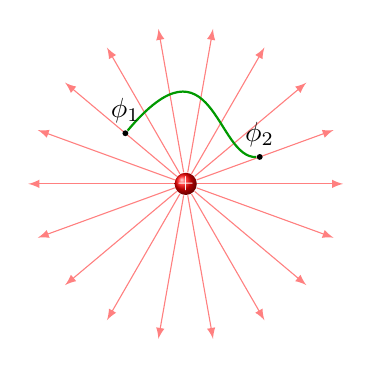
\begin{tikzpicture}[scale=1, transform shape, >=latex]
			\node [circle, ball color=red, inner sep=0pt, text=white,
				font=\scriptsize] (qp) at (0,0) {$+$};
			\foreach \i in {20,40,...,360}
				{
					\draw[->, red!50] (qp) -- ++(\i:2);
				}
			\node[circle, inner sep=0.75pt, fill] (1) at (140:1) {};
			\node[circle, inner sep=0.75pt, fill] (2) at (20:1) {};
			\draw [green!60!black, thick] (1) node[above, text=black] {$\phi_1$}  ..  controls
			(80:2) and
			(40:0.5) .. (2) node[above, text=black] {$\phi_2$};
		\end{tikzpicture}

	}
	%---------------------------------------------------------
	\captionbox{До поняття циркуляції вектора $\Efield$}[.45\linewidth]{

		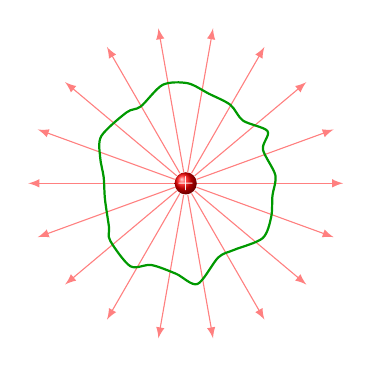
\begin{tikzpicture}[scale=1, transform shape,>=latex]
			\node [circle, ball color=red, inner sep=0pt, text=white,
				font=\scriptsize] (qp) at (0,0) {$+$};
			\foreach \i in {20,40,...,360}
				{
					\draw[->, red!50] (qp) -- ++(\i:2);
				}
			% distrorted sphere
			\pgfmathsetseed{2}
			\draw[green!60!black, thick] plot[domain=45:395,smooth cycle]
			(\x:{1+rnd*0.3});
		\end{tikzpicture}

	}
	%---------------------------------------------------------
\end{figure}
%=========================================================

Різницю потенціалів поля між точками $1$ і $2$ можна виразити через
напруженість \eqref{eq:Dphi}:
\begin{equation*}
	\int\limits_{(1)}^{(2)} \Efield\cdot d\vect{r} = \phi_1 - \phi_2 = -\Delta\phi.
\end{equation*}

Оскільки робота поля над зарядом не залежить від форми траєкторії ---
то для \emphx{довільної замкненої траєкторії $L$} маємо
\begin{equation}
	\tcbhighmath{
		\oint\limits_L \Efield\cdot d\vect{r}
		% \oint\limits_L \left( E_x dx + 	E_ydy + E_zdz \right)
		= 0
	}
\end{equation}
Цей інтеграл називається \emphx{циркуляцією вектора $\Efield$ по
	контуру $L$}, а рівність називається \emphx{теоремою про
	циркуляцію в інтегральній формі}.


%% --------------------------------------------------------
\subsection*{Теорема про циркуляцію в диференціальній формі}
%% --------------------------------------------------------


Нехай замкнутий контур $L(S)$ охоплює малу поверхню площею $S$. Вектор
$S$ спрямований за нормаллю до розглянутої площадки і за величиною
дорівнює площі цієї площадки: $\vect{S} = \vect{n}S$, $|\vect{n}| = 1$.
Напрямок вектора $\vect{S}$ задається позитивним напрямком обходу
контуру $L$ і визначається правилом гвинта.

\begin{SCfigure}[3.0][h!]
	\centering
	\begin{tikzpicture}[
                    scale=1.5,
                    >=latex,decoration={
					markings,
					mark=at position 0.75 with {\arrow{>}}}]
		\draw[postaction={decorate}, red, fill=red!10] (0,0) ellipse (1 and
		0.3);
		\draw[->, red] (0,0) -- ++(0,1) node[left] {$\vect{S}$};
		\draw[->, black, thick] (0,0) -- ++(0,0.5) node[right] {$\vect{n}$};
	\end{tikzpicture}
	\caption{Орієнтована площадка}
\end{SCfigure}


Коли контур стягується в точку:
$
	\lim\limits_{S\to0} \left( \frac1S \oint\limits_S \Efield\cdot
	d\vect{r}\right)  =
	(\Rot\Efield)_n
$
--- ця межа являє собою проекцію вектора $\Rot\Efield$ на напрямок нормалі
$\vect{n}$. З огляду на довільність вибору контуру робимо висновок, що:
\begin{equation*}
	\Rot\Efield \equiv \tcbhighmath{
		\rot\Efield = 0.
	}
\end{equation*}

\begin{Attention}
	Ротор вектора --- векторна величина!
\end{Attention}

\begin{problem}%
    Обчисліть ротор радіус-вектора.
\end{problem}

\begin{Attention}\small
    Ми розглянули перехід від циркуляції векторного поля по замкненому контуру до його ротору через аналіз малих площин у просторі. У математиці
    існує узагальнення цього принципу  для довільного векторного поля $\vect{A}$. Ця загальна теорема,
    відома як \emphx{теорема Стокса}, дозволяє пов'язати циркуляцію векторного поля вздовж замкненого контуру $L$ з поверхневим інтегралом від його
    ротора:
    \begin{equation}
       \oint\limits_L \vect{A} \cdot d\vect{r} = \iint\limits_S (\rot\vect{A}) \cdot d\vect{S}.
    \end{equation}
де $L$ --- замкнений контур, $S$ --- орієнтована поверхня, обмежена цим контуром, а $\vect{A}$ --- довільне векторне поле. Формула дозволяє переходити
від інтегральних форм до диференціальних.
\end{Attention}


%% --------------------------------------------------------
\subsection*{Потенціальні та вихрові поля}
%% --------------------------------------------------------

%=========================================================
\begin{figure}[h!]\centering
	%---------------------------------------------------------
	\begin{subfigure}[t]{0.45\linewidth}\centering
        \localinput{potential_field.tikz}
		\caption{Потенціальне поле}
		\label{tikz:potential_field}
	\end{subfigure}
	%---------------------------------------------------------
	\begin{subfigure}[t]{0.45\linewidth}\centering
        \localinput{curl_field.tikz}
		\caption{Вихрове поле}
		\label{tikz:curl_field}
	\end{subfigure}
	%---------------------------------------------------------
	\caption{Приклад силових ліній потенціального та вихрового полів}
    \label{tikz:source_and_curl_field}
\end{figure}
%=========================================================

Лінії поля або десь починаються і десь закінчуються, або є замкнутими. Так, наприклад, заряди створюють електричне поле, лінії якого починаються або
закінчуються на цих зарядах (або в нескінченності). Далі в курсі ми познайомимось з магнітним полем, та навіть з електричним полем, яке не створюється
зарядами. Лінії таких полів є замкненими.  Точки, в якій лінії поля починаються (або закінчуються), називається \emphx{джерелом (або стоком) поля}.
Точка, навколо якої замикаються лінії поля, називається \emphx{вихором поля}. Поля, які мають джерела, називаються потенціальними, а ті які мають вихори
--- вихровими. (риc.~\ref{tikz:source_and_curl_field}).



%Якщо лінії поля або десь \emphx{починаються} і десь \emphx{закінчуються}
%--- тобто мають витоки та стоки --- такі поля називаються
%\emphx{потенціальними} (рис.~\ref{tikz:potential_field}).
%
%Якщо лінії поля є \emphx{замкненими} --- тобто \emphx{НЕ мають витоків та стоків}
%--- такі поля називаються \emphx{вихровими} (рис.~\ref{tikz:curl_field}).




%% --------------------------------------------------------
\section{Граничні умови}
%% --------------------------------------------------------



На границі розділу двох середовищ електричне поле може змінюватися стрибком, але цей стрибок залишається скінченним. Такі \emphx{стрибки називаються
розривами першого роду}. Іншими словами, значення електричного поля з одного боку границі відрізняється від значення з іншого боку, але саме поле не стає
нескінченним і не зникає на самій поверхні.

\begin{SCfigure}[0.5][h!]
	\centering
	\localinput{bc1.tikz}
	\caption{До виведення першої граничної умови}%
    \label{tikz:bc1}
\end{SCfigure}

Застосуємо теорему Гаусса до поверхні $S$ нескінченно малого циліндра, що охоплює частину межі
розділу двох
середовищ (рис.~\ref{tikz:bc1}). Оскільки $d\vect{S}_1 = - d\vect{S}_2$, $q = \sigma dS$,
$d\vect{S}_2 =
	\vect{n}\ dS$,
маємо

\begin{equation*}
	\oiint\limits_S \Efield\cdot d\vect{S} = 4\pi\sigma\ \Rightarrow  \Efield_1\cdot
	d\vect{S}_1 +
	\Efield_2\cdot d\vect{S}_2 \equiv (\Efield_2 - \Efield_1)\cdot\vect{n}\ dS  = 4\pi\sigma dS
\end{equation*}


Звідси випливає перша гранична умова:
\begin{equation}
	\tcbhighmath{
		E_{2n} - E_{1n} = 4\pi\sigma.
	}
\end{equation}

Нормальна складова вектора $\Efield$ зазнає стрибка при
переході через заряджену границю розділу. Однак якщо заряди на межі розділу відсутні
($\sigma =
	0$), то $E_{1n} = E_{2n}$ і стрибка не буде.


\begin{SCfigure}[0.5][h!]
	\centering
	\localinput{bc2.tikz}
	\caption{До виведення другої граничної умови}%
    \label{tikz:bc2}
\end{SCfigure}
Застосуємо теорему про циркуляцію до нескінченно малого прямокутного
контуру $L$, що проходить на нескінченно малій відстані над і під поверхнею
розділу середовищ (рис.~\ref{tikz:bc2}). Оскільки $d\vect{r}_2 = - d\vect{r}_1$, позначимо $d\vect{r} = d\vect{r}_2  = \vect{\tau} d\ell$ маємо:

\begin{equation*}
	\oint\limits_L \Efield\cdot d\vect{r} = 0 \Rightarrow \Efield_1\cdot d\vect{r}_1 +
	\Efield_2\cdot d\vect{r}_2 \equiv (\Efield_2 - \Efield_1)\cdot d\vect{r} \equiv (\Efield_2 - \Efield_1)\cdot \vect{\tau} d\ell = 0,
\end{equation*}
де $\vect{\tau}$ --- це одиничний вектора, дотичний до поверхні розділу, $d\ell$ --- елемент контура.

Звідси випливає друга гранична умова $(\Efield_2 - \Efield_1)\cdot \vect{\tau} = 0$, або еквівалентна форма:
\begin{equation}
	\tcbhighmath{
		E_{1\tau} = E_{2\tau}.
	}
\end{equation}


Тангенціальна складова $\Efield$ виявляється однаковою по обидва боки границі розділу (не
зазнає стрибка).

%% --------------------------------------------------------
\section{Рівняння Пуассона та Лапласа}
%% --------------------------------------------------------

Оскільки $\Efield = - \vect{\nabla}\phi$ і $\divg\Efield  = 4\pi\rho$, то
звідси випливає \emphx{рівняння Пуассона для потенціалу поля}:
\begin{equation*}
	\tcbhighmath{
		\nabla^2\phi = - 4\pi\rho.
	}
\end{equation*}

\begin{Attention}
Тут введено оператор Лапласа (лапласіан)
\begin{equation*}
	\nabla^2 = \frac{\partial^2}{\partial x^2} +
	\frac{\partial^2}{\partial y^2} + \frac{\partial^2}{\partial z^2}.
\end{equation*}
\end{Attention}


У області простору, вільній від зарядів ($\rho = 0$ ), рівняння Пуассона
зводиться до \emphx{рівняння Лапласа}
\begin{equation*}
	\tcbhighmath{
		\nabla^2\phi = 0 .
	}
\end{equation*}

Як і будь-яке рівняння в часткових похідних, рівняння Пуассона та Лапласа допускають безліч лінійно незалежних часткових розв'язків. Однак, у конкретній
фізичній задачі додатково задаються граничні умови (наприклад, значення потенціалу $\phi$ на поверхні, що обмежує область, та/або нормальна компонента
напруженості електричного поля). Ці умови визначають задачу однозначно. Таким чином, будь-який розв’язок, що задовольняє рівнянню Пуассона або Лапласа і
відповідає граничним умовам, буде єдино можливим.
Дійсно, якщо при заданих граничних умовах розв'язок не один, то це означатиме, що буде не один електричний
<<ландшафт>>, отже, у кожній точці поле $\Efield$ також буде неоднозначним --- що є
фізично абсурдним. Це твердження називають \emphx{теоремою єдиності}. Теоремою єдиності можна скористатись, коли нам треба <<вгадати>> розв'язок
рівняння Пуассона (або Лапласа). Якщо розв'язок задачі задовольняє рівнянню Лапласа (або Пуассона) і граничним умовам, то можна стверджувати, що воно є
правильним і єдиним, навіть якщо ми його вгадали.




%=========================================================
\begin{problem}%
Використовуючи теорему Гаусса в диференціальній формі знайдіть напруженість та потенціал
електричного поля всередині та зовні однорідно зарядженої кулі. Заряд кулі дорівнює
$Q$, радіус кулі~$R$.
\end{problem}

